\chapter{Anvendelsesgrænsetilstand}
I det følgende afsnit bestemmes anvendelsesgrænsetilstanden for tilbygningen til Strøybergs Palæ. Ud fra anvendelsesgrænsetilstanden kan det vurderes, om bygningen har tilstrækkelig små deformationer til, at dimensioner kan godtages. 
\newline \indent{     }  Jævnført Eurocode 1993, afsnit 7.2, beregnes anvendelsesgrænsetilstanden kun for én variabel last, hvilken vælges til at være vindlasten. Denne last forlænges helt ned til understøtningerne, og der ses bort fra jordlasten. Derfor er der udregnet nye reaktioner for konstruktionen, som er vist på Figur \ref{fig:snitanvendelse}. Udregningerne findes i BILAG XX. 

\section{Moment}
Ved udbøjning skal bjælkens differentialligning anvendes, og derfor skal momentligningen for hvert snit bruges. Udbøjningen beregnes ud fra hovedkonstruktionens stålstænger, hvor der laves fem snit, som vist på Figur \ref{fig:snitanvendelse}. Dog ses der bort fra den højre del af konstruktionen, og dermed er det kun snit 1-3 der anvendes.

\begin{figure}[H]
	\centering
	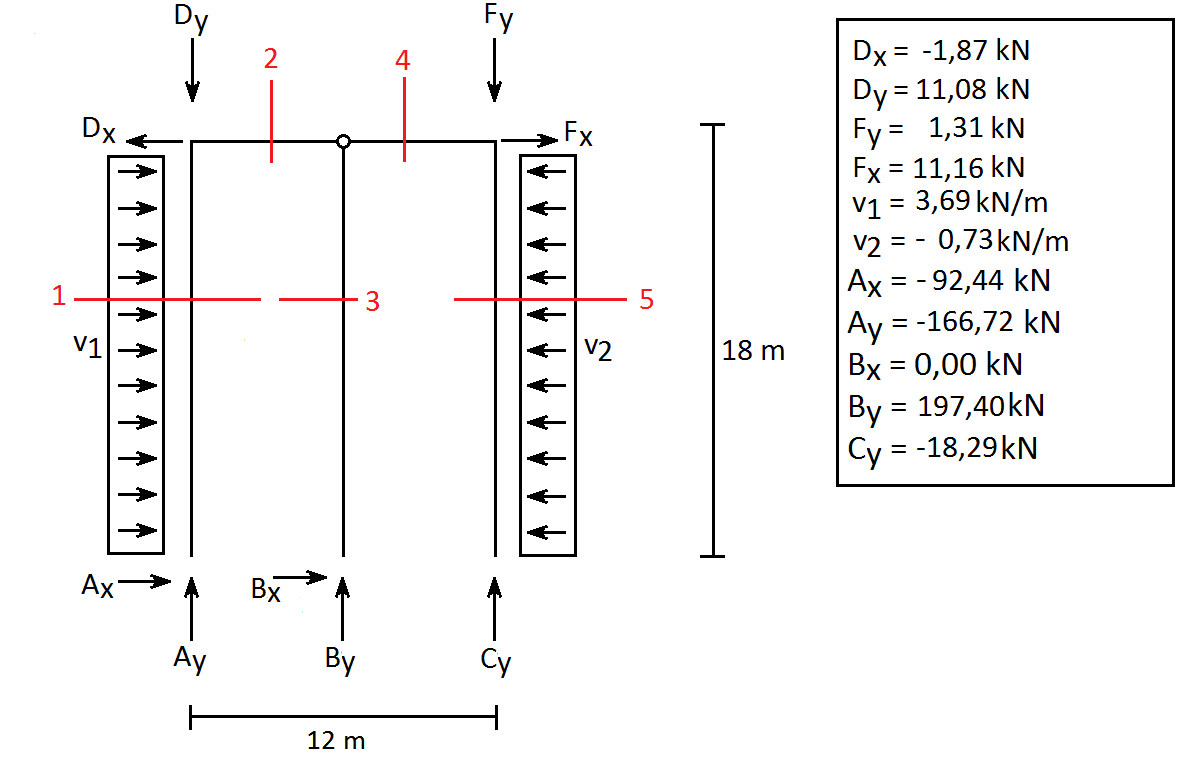
\includegraphics[width=0.9\textwidth]{billeder/snitanvendelse.png}
	\caption{Snit}
	\label{fig:snitanvendelse}
\end{figure}

Nedenfor er vist et eksempel på, hvordan momentligningen regnes for snit 1. Alle beregningerne findes i Bilag XX.
\newline
\newline
\textbf{Snit 1: 0 m < $x_1$ < 18 m}
\newline
Fritlegemediagrammet for snit 1 ses på Figur \ref{fig:snitetan}. LAV NYT BILLEDE!
\begin{figure}[H]
	\centering
	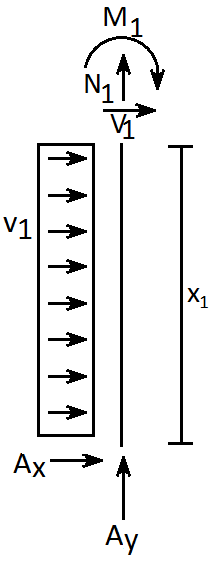
\includegraphics[width=0.2\textwidth]{billeder/asnitet.png}
	\caption{Snit 1}
	\label{fig:snitetan}
\end{figure}

\begin{equation}
PILE PÅ! (POS MED URET)  0 = M_1 + A_xx_1 + v_1x_1 \frac{x}{2}
\\
M_1(x_1)= {-A_x x_1-\frac{1}{2}v_1x_1^2}
\end{equation}

Følgende momentligninger fås for snit 1, 2 og 3, og disse kaldes $M_1$, $M_2$ og $M_3$:
\begin{equation}
	M_1(x_1)= -A_xx_1-\frac{1}{2}v_1x_1^2 = v''EI
\end{equation}

\begin{equation}
	M_2(x_2)= -v_1 \cdot 162m^2 - A_x \cdot 18m + A_yx_2 - P_1y x_2^2 = v''EI
\end{equation}

\begin{equation}
	M_3(x_3)= B_xx_3 = v''EI
\end{equation}

\section{Bjælkens differentialligning}
Nu skal bjælkens differentialligning anvendes. Da det statiske system for tilbygningen til Strøybergs Palæ er statisk bestemt, er det den anden ordens afledede, som anvendes for at bestemme udbøjningerne.

For $M_1$ bestemmes nu den første afledede $alpha_1$ og anden aflede $u_1$: %Her vises integration%
\begin{equation}
	\int \frac{M_1(x_1)}{EI} = \int \frac{-A_x x_1 - \frac{1}{2}\cdot v_1 x_1^2}{EI}
	= \alpha_1(x_1) = \frac{-\frac{1}{2} A_x x_1^2 - \frac{1}{6}  v_1  x_1^3 }{EI} + k_1
\end{equation}

\begin{equation}
	\int \alpha_1(x_1) = \int \frac{-\frac{1}{2} A_x x_1^2 - \frac{1}{6} v_1 x_1^3}{EI} + k_1
	= u_1(x_1) = \frac{-\frac{1}{6} A_x x_1^3 - \frac{1}{24} v_1x_1^4 }{EI} + k_1 x_1 + k_2
\end{equation}

Det samme gøres for $M_2$ og $M_3$, hvilket giver følgende funktioner for den første og anden afledede: 
\newline
\newline
$M_2$:
\begin{equation}
	\alpha_2(x_2) = \frac{-v_1 \cdot 162m^2 \cdot x_2 - A_x \cdot 18m \cdot x_2 + \frac{1}{2} A_y x_2^2 - \frac{1}{2}P_1y x_2^2}{EI} + k_3
\end{equation}
	
\begin{equation}
	u_2(x_2) = \frac{-v_1 \cdot 81m^2 x_2^2 - A_x \cdot 9m \cdot x_2^2 + \frac{1}{6} A_y x_2^3 - \frac{1}{6} P_1y x_2^3}{EI} + k_3 x_2 + k_4
\end{equation} 
\newline
\newline
$M_3$:
\begin{equation}
\alpha_3(x_3) = \frac{1}{2}\frac{B_x x_3^2}{EI} + k_5
\end{equation}

\begin{equation}
u_3(x_3) = \frac{1}{6} \frac{B_x x_3^3}{EI} + k_5 x_3 + k_6
\end{equation}

Ved integrering af ligningningerne giver dette 6 ligningner med 6 ubekendte konstanter. Disse bestemmes ved at opstille 6 randbetingelser for det statiske system: 

\begin{table}[h]
	\begin{tabular}{l}
		$u_1(0)=0$       \\
		$\alpha_1(h)$=$\alpha_2(0)$ \\
		$u_1(h)$=$u_3(h)$ \\
		$u_2(h)$=0       \\
		$u_2(l)$=0       \\
	\end{tabular}
\end{table}

De opsatte randbetingelser løses, og de 6 konstanter får værdierne: 

\begin{table}[h]
	\begin{tabular}{l}
		$k_1 = -0,\!14$       \\
		$k_2 = 0$             \\
		$k_3 = -0,\!02$       \\
		$k_4 = 0$             \\
		$k_5 = -0,\!10$       \\
		$k_6 = 0$             \\ 
	\end{tabular}
\end{table}

Udregningerne for konstanterne findes i bilag XX!
\newline
\newline 
Konstanterne indsættes nu i formlerne for $u_1(x_1)$, $u_2(x_2)$ og $u_3(x_3)$, og ud fra de nye funktioner kan udbøjningen bestemmes.
\begin{equation}
u_1(18m) = -1,\!76 m
\end{equation}

\begin{equation}
u_2(3m) = -0,\!02 m
\end{equation}

\begin{equation}
u_3(18m) = -1,\!76 m.   
\end{equation}

TEGN EN UDBØJNINGSKURVE FOR KONSTRUKTIONEN? 

Disse udbøjninger skal nu sammenlignes med de maksimalt tilladte udbøjninger for en bærende konstruktion, som findes i Eurocode 1993, afsnit 7.2. 

Maksimal vandret udbøjning: 
\begin{equation}
\frac{h_3}{500}
\\
\frac{18000mm}{500} = 36 mm
\end{equation}

Maksimal lodret udbøjning
\begin{equation}
\frac{l}{400}
\\
\frac{6000mm}{400} = 15 mm
\end{equation}
